
%-----------------------------------------------------------------------------
% Chapter:The Course2018 LMS 
%-----------------------------------------------------------------------------

\chapter{The Course2018 LMS}
\label{chap:RSLT}

This chapter shows the result of the project by providing screenshots for
each of the modules in the \emph{Course2018} LMS.

\section{User authentication}
The Login interface, shown in Figure~\ref{fig:LOGIN}, is used for authentication
of all users.
\begin{figure}[H]
    \centering
        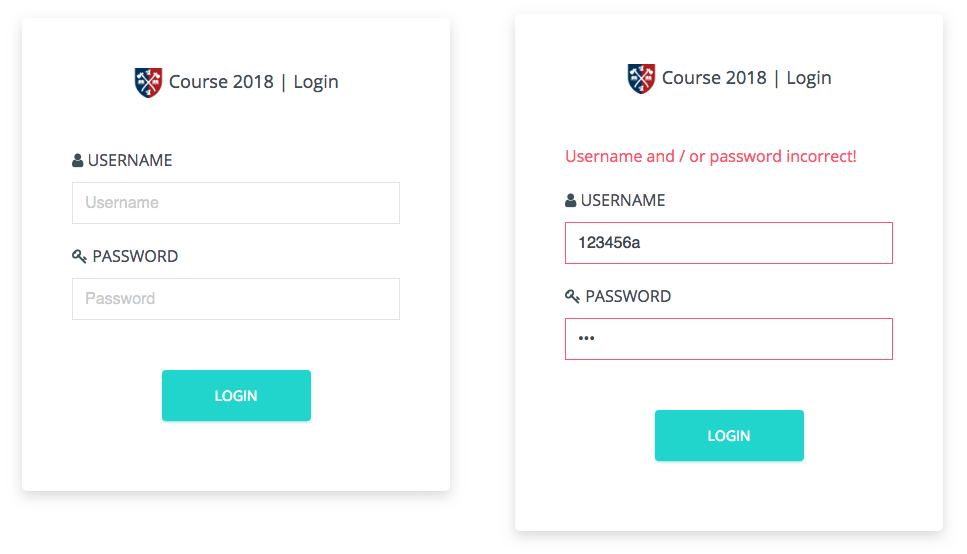
\includegraphics[width=.9\textwidth]{figures/login}
    \caption{System login interface}
    \label{fig:LOGIN}
\end{figure}

\section{Course management}

\subsection{Create courses}
The form shown in Figure~\ref{fig:NEW_COURSE} is used by instructors to create
courses in the \emph{Course\-2018} LMS.

\begin{figure}[H]
    \centering
        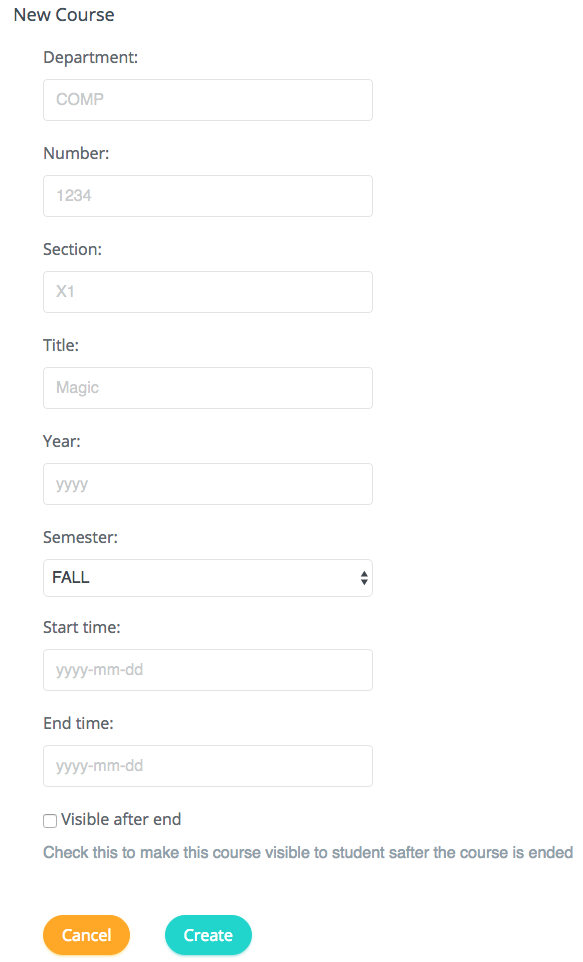
\includegraphics[width=.6\textwidth]{figures/create-courses}
    \caption{Create course interface}
    \label{fig:NEW_COURSE}
\end{figure}

\subsection{Course summary}
Figure~\ref{fig:COURSE_SUMMARY} shows the course summary interface in which
instructors can view the latest assignment grade summary, marking status,
student activities, as well as manage the course (e.g., register TAs, shown
in Figure~\ref{fig:REG_TA}).

\begin{figure}[H]
    \centering
        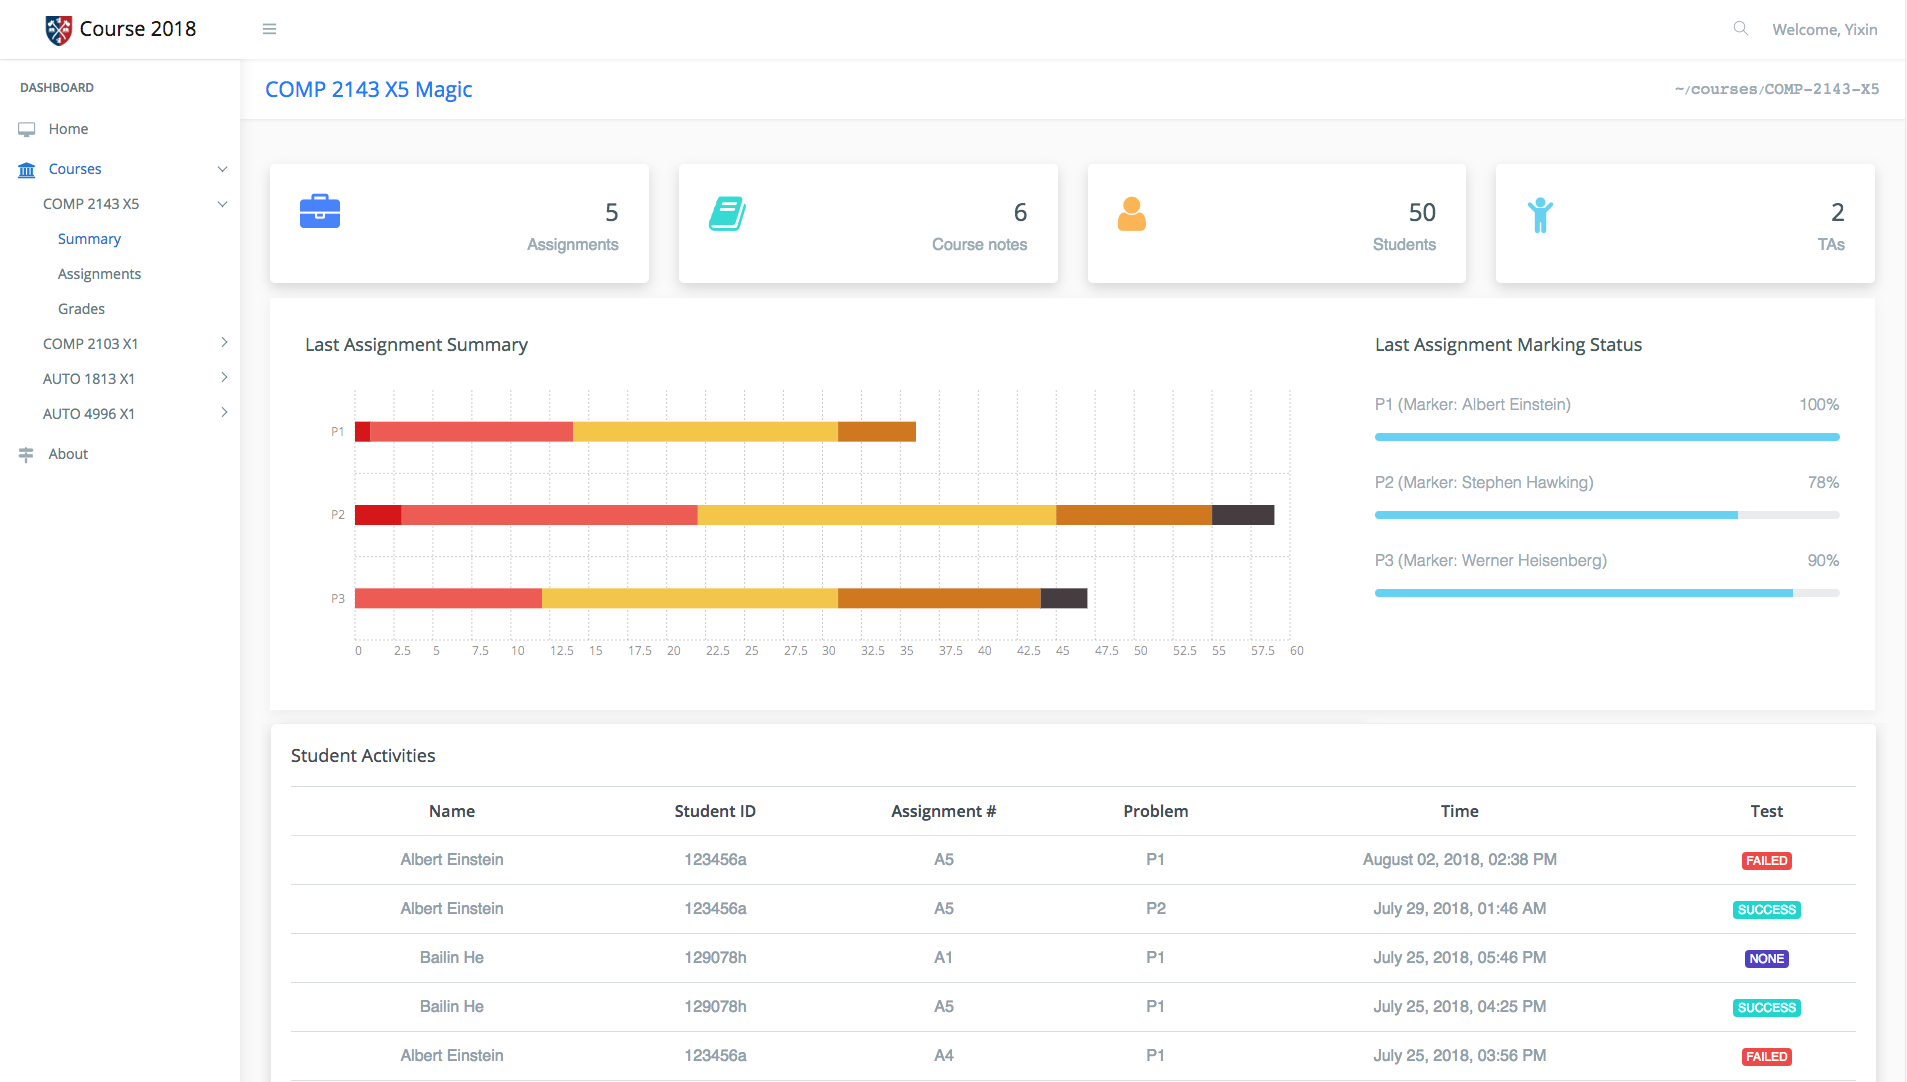
\includegraphics[width=1.0\textwidth]{figures/course-summary}
    \caption{Course summary interface}
    \label{fig:COURSE_SUMMARY}
\end{figure}

\begin{figure}[H]
    \centering
        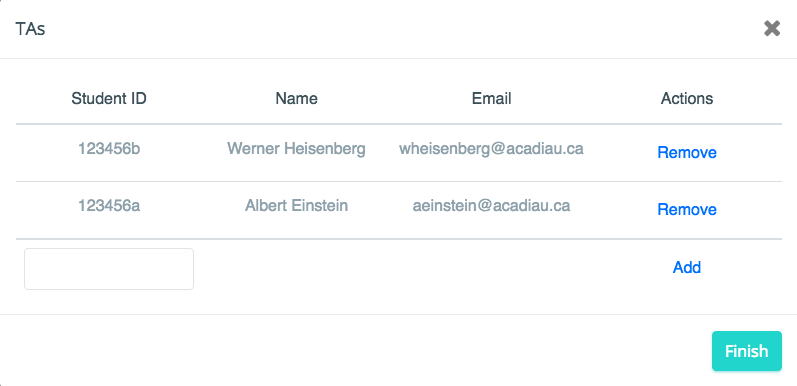
\includegraphics[width=0.8\textwidth]{figures/reg-ta}
    \caption{TA registration interface}
    \label{fig:REG_TA}
\end{figure}


\section{Assignment management}

\subsection{Create assignments}
The form shown in Figure~\ref{fig:NEW_ASM} is used by instructors to create
assignments for a course.

\begin{figure}[H]
    \centering
        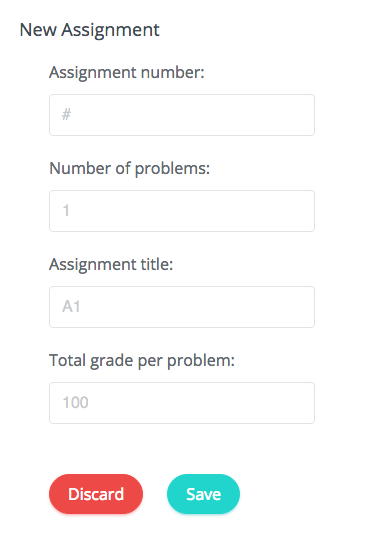
\includegraphics[width=0.4\textwidth]{figures/create-asm}
    \caption{Create assignment interface}
    \label{fig:NEW_ASM}
\end{figure}

\subsection{Assignment summary}

\subsubsection{Professor view}
Figure~\ref{fig:ASM_SUMMARY_PROF} shows the assignment summary interface for
instructors to view the submission status of the latest assignment, manage
each individual assignment, and release assignment feedback to the students.

\subsubsection{Student view}
The student's assignment summary interface, shown in
Figure~\ref{fig:ASM_SUMMARY_STUDENT}, contains a table of a list
of assignments with links to the detail page of each individual assignment.

\pagebreak

\begin{figure}[H]
    \centering
        \includegraphics[width=1.0\textwidth]{figures/asm-summary-prof}
    \caption{Assignment summary interface for instructors}
    \label{fig:ASM_SUMMARY_PROF}
\end{figure}

\begin{figure}[H]
    \centering
        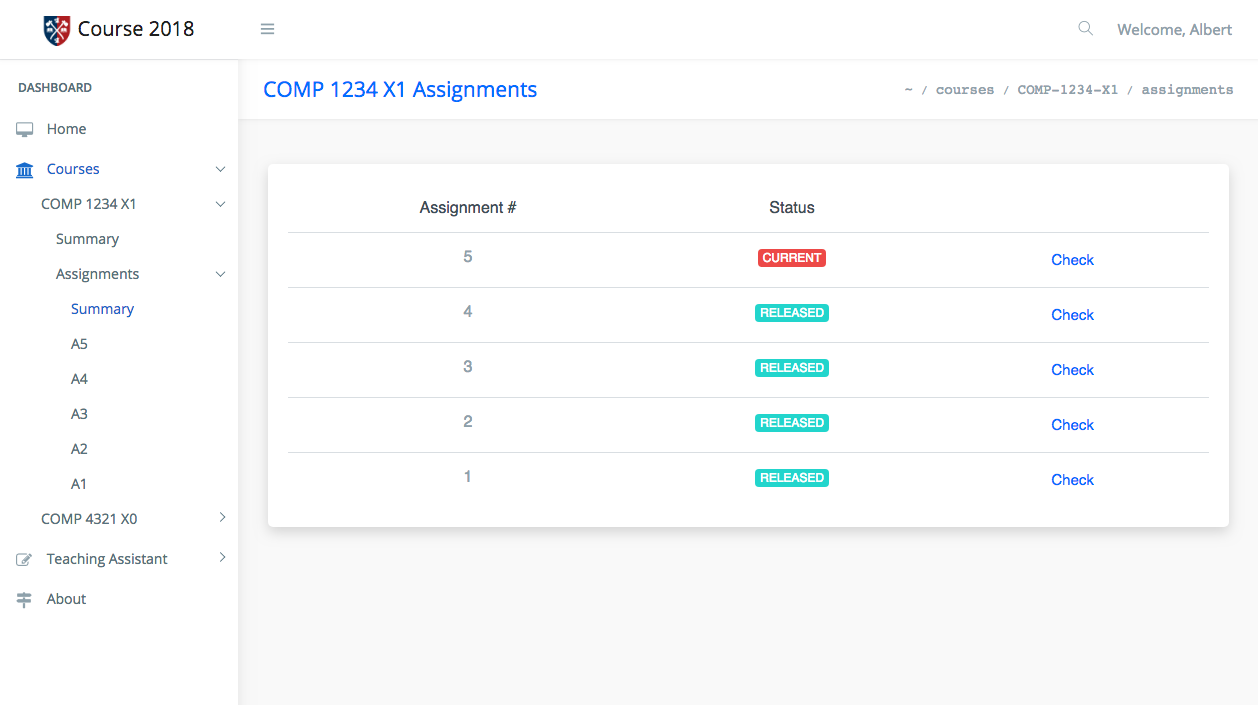
\includegraphics[width=1.0\textwidth]{figures/asm-summary-student}
    \caption{Assignment summary interface for students}
    \label{fig:ASM_SUMMARY_STUDENT}
\end{figure}

\pagebreak

\subsection{Assignment detail}

\subsubsection{Professor view}
The assignment detail interface for instructors contains the following three
sections:

\begin{enumerate}
    \item \textbf{Submits}: all submissions of an assignment are displayed
        in a table with links so that instructors can view and grade each
        student's assignment; a drop-down menu is also provided to assign TAs
        to different problems (shown in Figure~\ref{fig:ASM_SUBMITS}).
    \item \textbf{Manage}: the form shown in Figure~\ref{fig:ASM_MANAGE} is
        presented to the instructor in this section
        to modify the detail information of an assignment, as well as to
        manage assignment attachments.
    \item \textbf{Auto Run}: a form (see Figure~\ref{fig:ASM_AUTORUN}) is
        presented to the instructor in this
        section to modify the configurations of the assignment's automated
        test scheme and test cases.
\end{enumerate}

\begin{figure}[H]
    \centering
        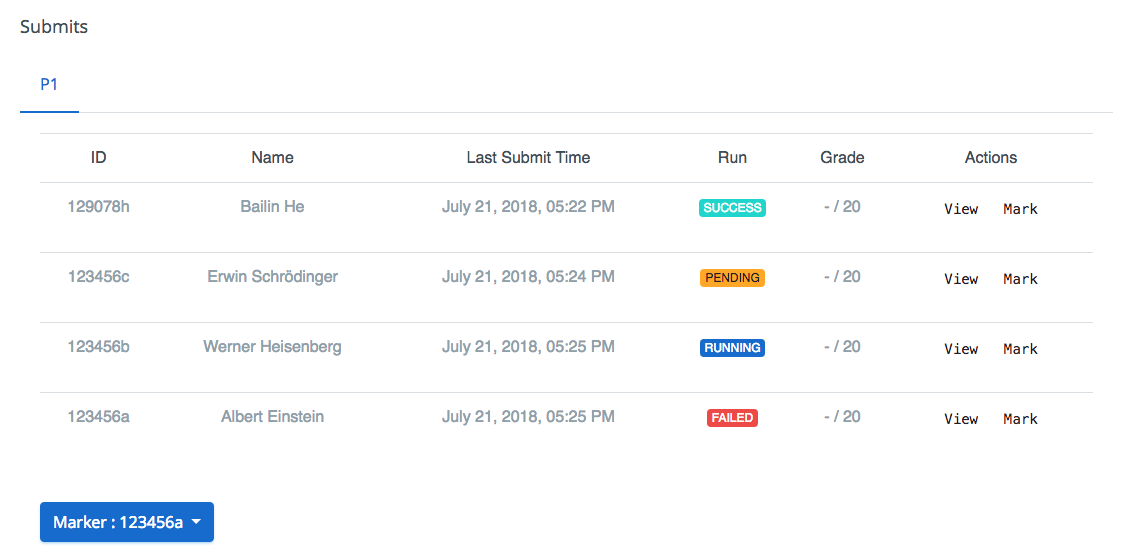
\includegraphics[width=1.0\textwidth]{figures/asm-submits}
    \caption{Assignment submissions interface}
    \label{fig:ASM_SUBMITS}
\end{figure}

\begin{figure}[H]
    \centering
        \includegraphics[width=1.0\textwidth]{figures/asm-manage}
    \caption{Assignment management interface}
    \label{fig:ASM_MANAGE}
\end{figure}

\begin{figure}[H]
    \centering
        \includegraphics[width=0.95\textwidth]{figures/asm-autorun}
    \caption{Assignment automated test configurations interface}
    \label{fig:ASM_AUTORUN}
\end{figure}

\subsubsection{Student View}
The student's assignment detail view is composed of a tab panel where users can
select to view the detail and attachments of an assignment, or submit files
to different problems of an assignment (shown in Figure~\ref{fig:ASM_DETAIL}
and Figure~\ref{fig:ASM_PROBLEM}).

\begin{figure}[H]
    \centering
        \includegraphics[width=1.0\textwidth]{figures/asm-detail}
    \caption{Assignment detail interface for students}
    \label{fig:ASM_DETAIL}
\end{figure}

\begin{figure}[H]
    \centering
        \includegraphics[width=1.0\textwidth]{figures/asm-problem}
    \caption{Assignment problem interface for students}
    \label{fig:ASM_PROBLEM}
\end{figure}


\section{File management and display}

The interface shown in Figure~\ref{fig:FILE_UPLOAD} is used for uploading
attachments (by instructors) and submitting assignments (by students), as well
as management (delete, modify) of those files.

\begin{figure}[H]
    \centering
        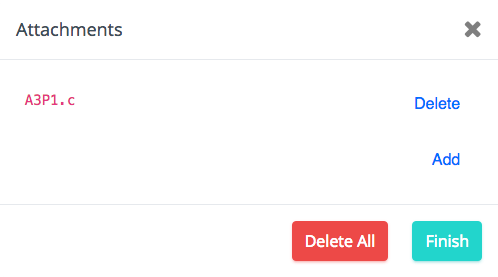
\includegraphics[width=0.7\textwidth]{figures/file-upload}
    \caption{File upload interface}
    \label{fig:FILE_UPLOAD}
\end{figure}

Whenever a user wishes to view a file, the interface shown in
Figure~\ref{fig:VIEW_FILE} is presented to the user. If source code management
(\emph{Git}) is enabled for the assignment, a \emph{Diff} button is displayed;
and the user can click on it to view the changes between the two latest
version of a file, as shown in Figure~\ref{fig:VIEW_FILE_DIFF}.

\begin{figure}[H]
    \centering
        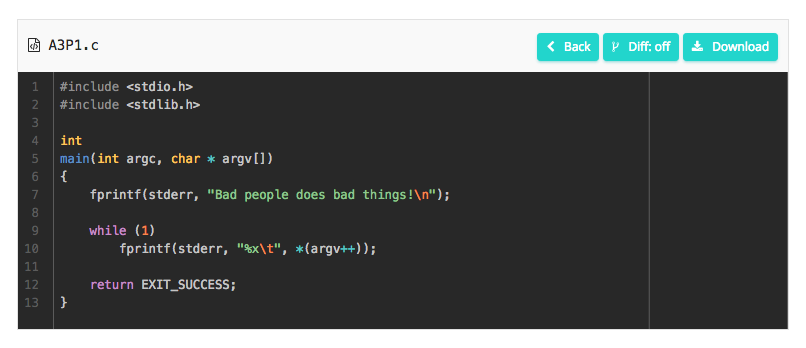
\includegraphics[width=1.0\textwidth]{figures/view-file}
    \caption{File upload interface}
    \label{fig:VIEW_FILE}
\end{figure}

\begin{figure}[H]
    \centering
        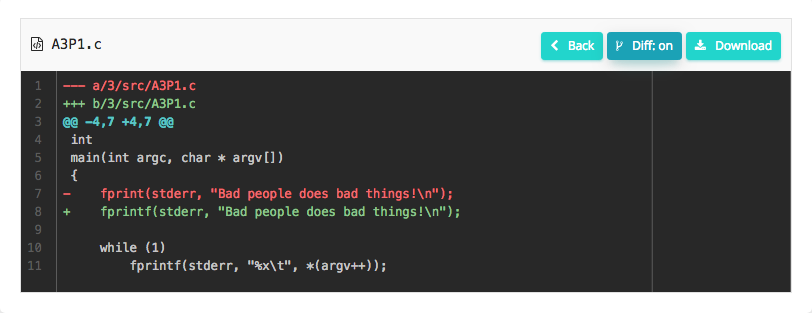
\includegraphics[width=1.0\textwidth]{figures/view-file-diff}
    \caption{File upload interface}
    \label{fig:VIEW_FILE_DIFF}
\end{figure}


\section{Automated test}
As it is shown in Figure~\ref{fig:ASM_SUBMITS} and Figure~\ref{fig:ASM_PROBLEM},
a test status badge is displayed on each submission. This badge is clickable
with a link to an interface that displays the test result
(Figure~\ref{fig:TRACE}).

\begin{figure}[H]
    \centering
        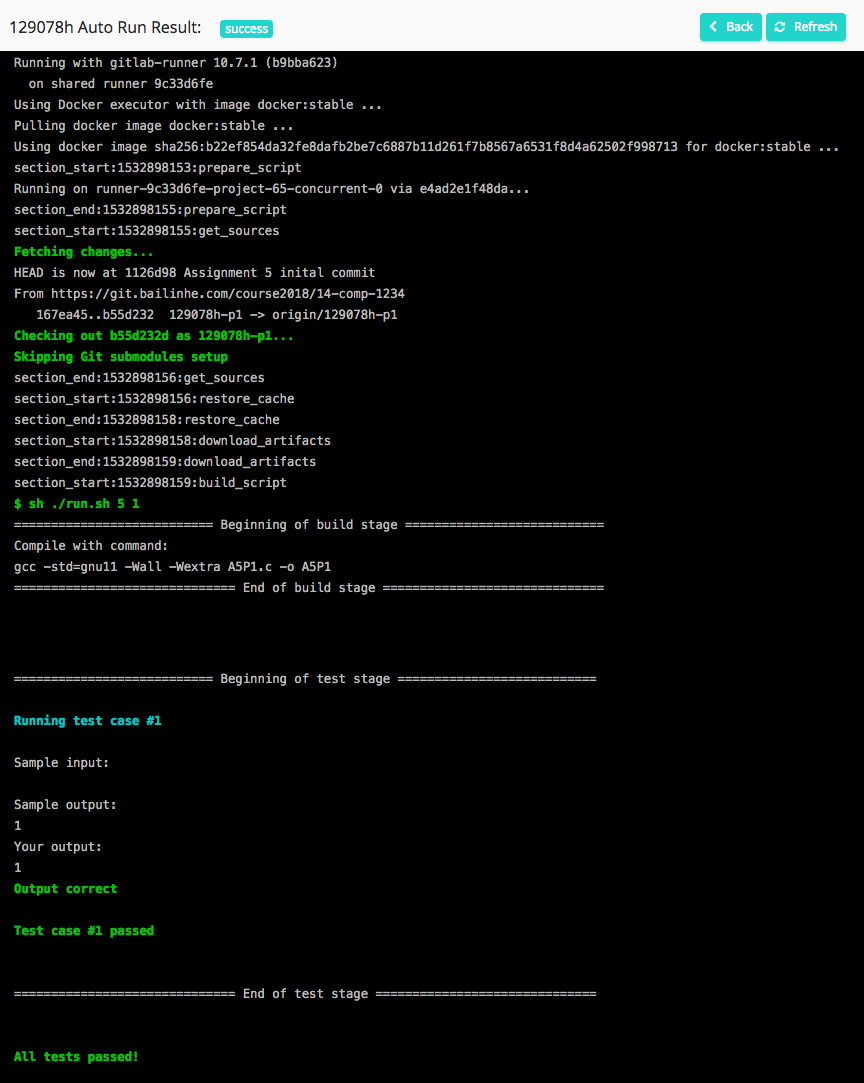
\includegraphics[width=0.85\textwidth]{figures/job-trace}
    \caption{Automated test result interface}
    \label{fig:TRACE}
\end{figure}

If the automated test scheme is updated after a job is finished, a notification
is presented to the user to re-run the test~(Figure~\ref{fig:RERUN}).

\begin{figure}[H]
    \centering
        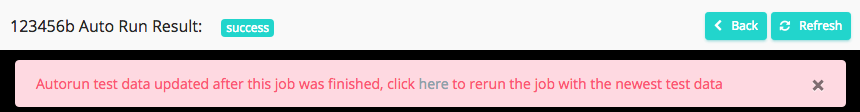
\includegraphics[width=1.0\textwidth]{figures/rerun}
    \caption{Automated test result re-run notification}
    \label{fig:RERUN}
\end{figure}

\section{Marking interface}
\subsection{Marker's view}
The marking interface for markers (i.e., instructors and TAs) is shown in
Figure~\ref{fig:MARKING}. The grade which appears at the upper left corner can
be automatically calculated and updated according to the comments that are
entered in the editor.

\begin{figure}[H]
    \centering
        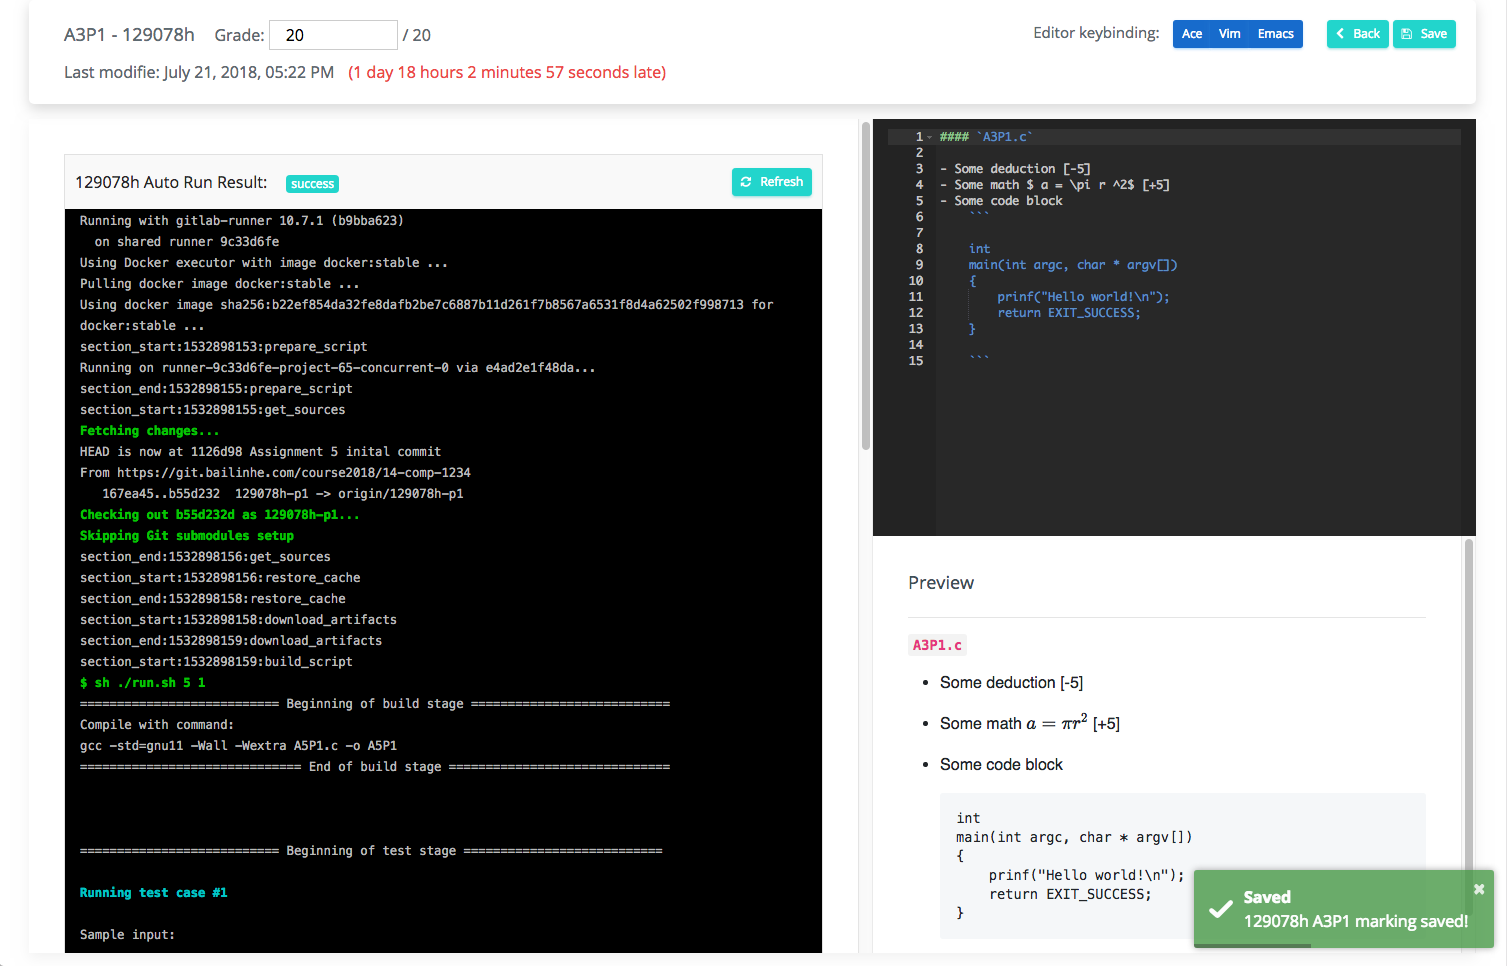
\includegraphics[width=0.95\textwidth]{figures/marker}
    \caption{Marking interface for instructors and TAs}
    \label{fig:MARKING}
\end{figure}

\subsection{Student's view}
The assignment feedback interface for students is shown in
Figure~\ref{fig:FEEDBACK}.
The files of the student's assignment are displayed on the left-hand side,
whereas the TA or instructor's feedback are displayed on the right-hand side,
so that the student can easily refer the comments to his own assignment.

\begin{figure}[H]
    \centering
        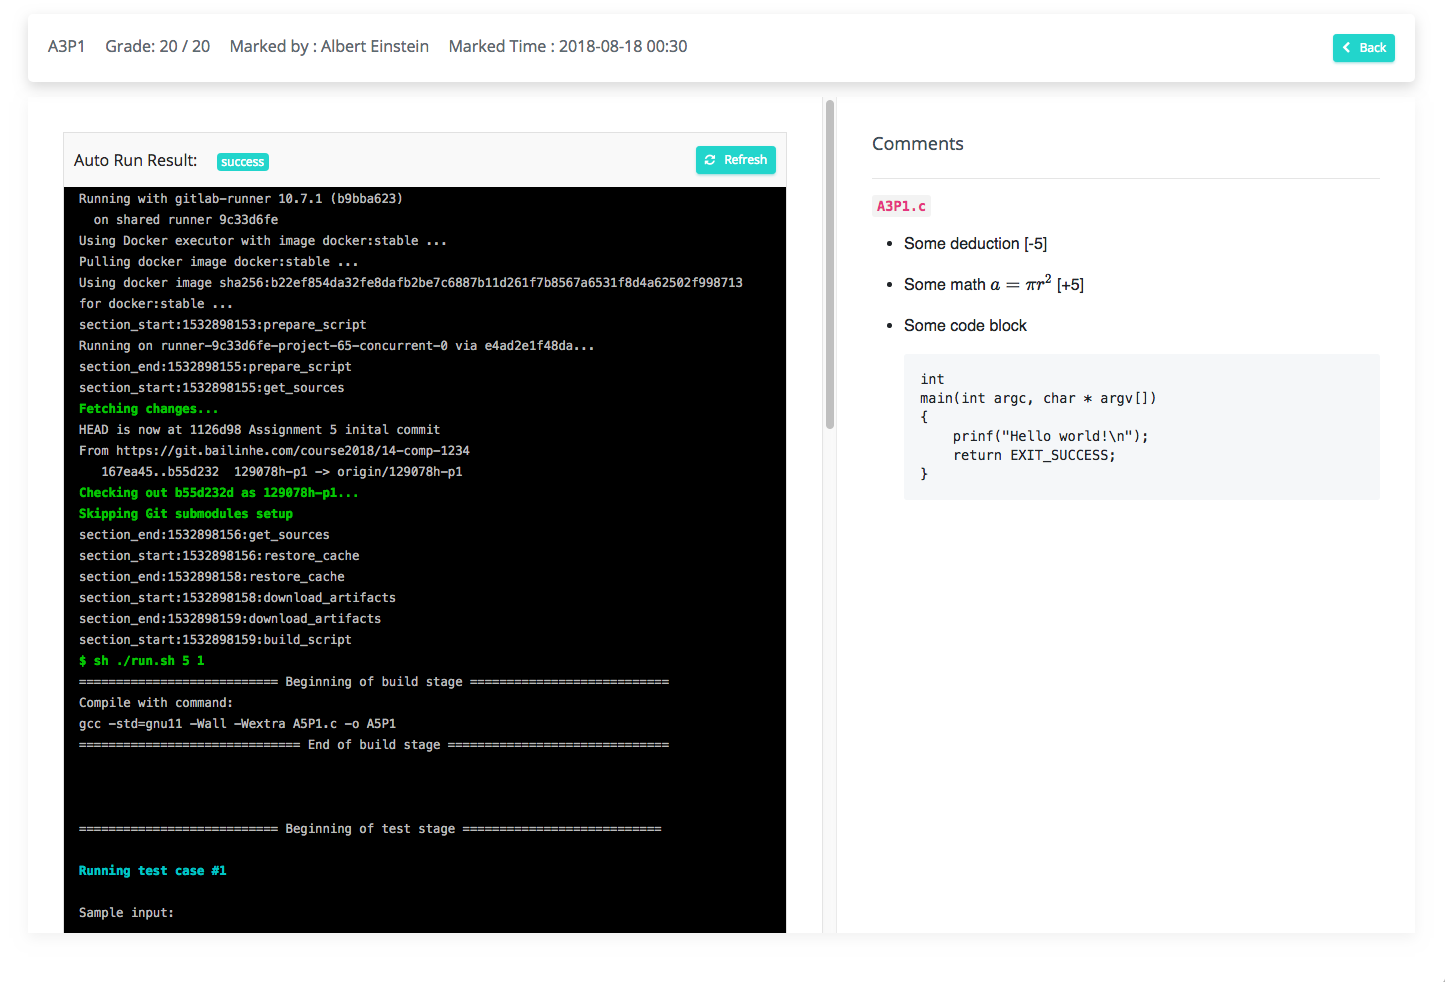
\includegraphics[width=1.0\textwidth]{figures/feedback}
    \caption{Assignment feedback interface for students}
    \label{fig:FEEDBACK}
\end{figure}